\begin{frame}[fragile]
    \frametitle{Geometry I}
    \inputminted[frame=single,fontfamily=tt,fontsize=\footnotesize]{python}{examples/geom1.py}
\end{frame}

\begin{frame}\frametitle{Geometry I: plots}
    \begin{columns}
        \column{0.3\textwidth}
            {\tiny z plane}
            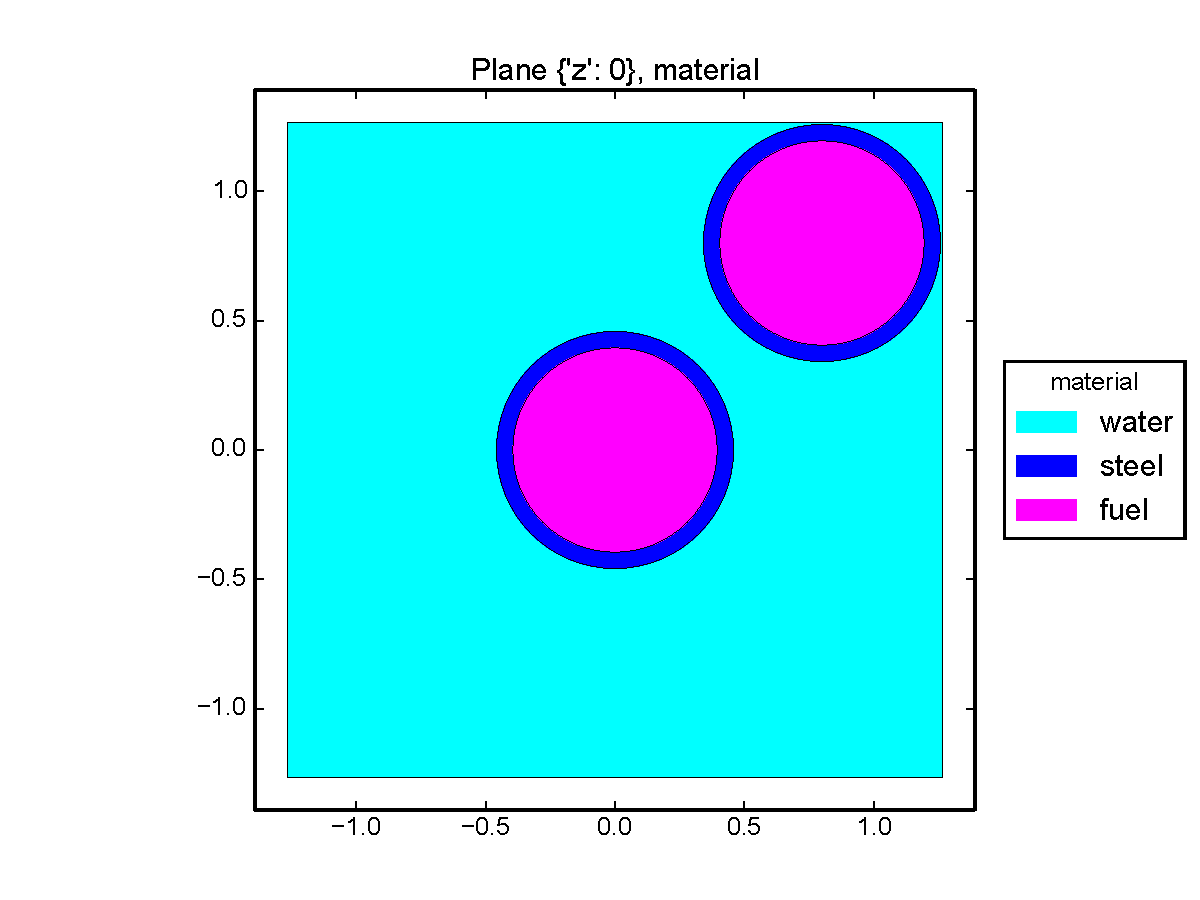
\includegraphics[width=\textwidth]{examples/geom1_pz.pdf}
        \column{0.3\textwidth}
            {\tiny x plane}
            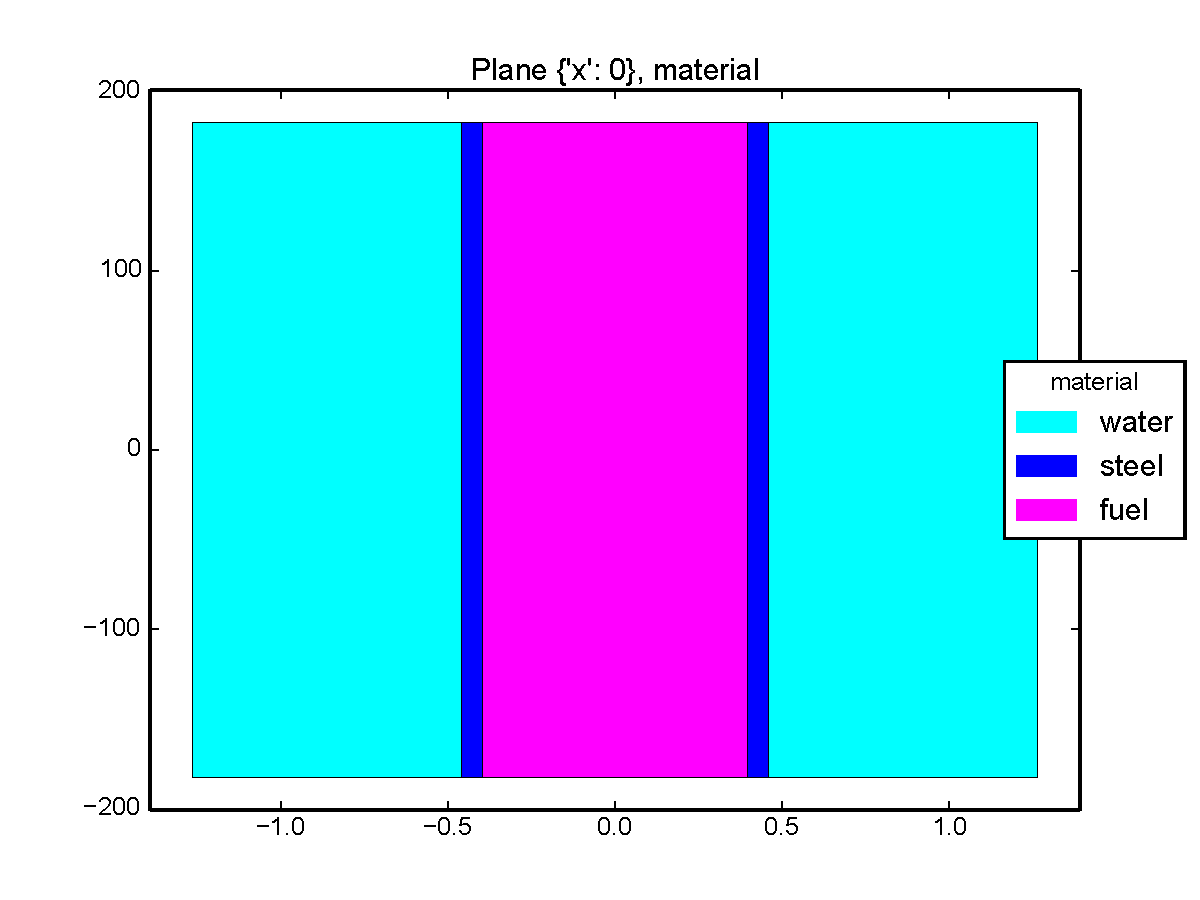
\includegraphics[width=\textwidth]{examples/geom1_px.pdf}
        \column{0.3\textwidth}
            {\tiny y plane}
            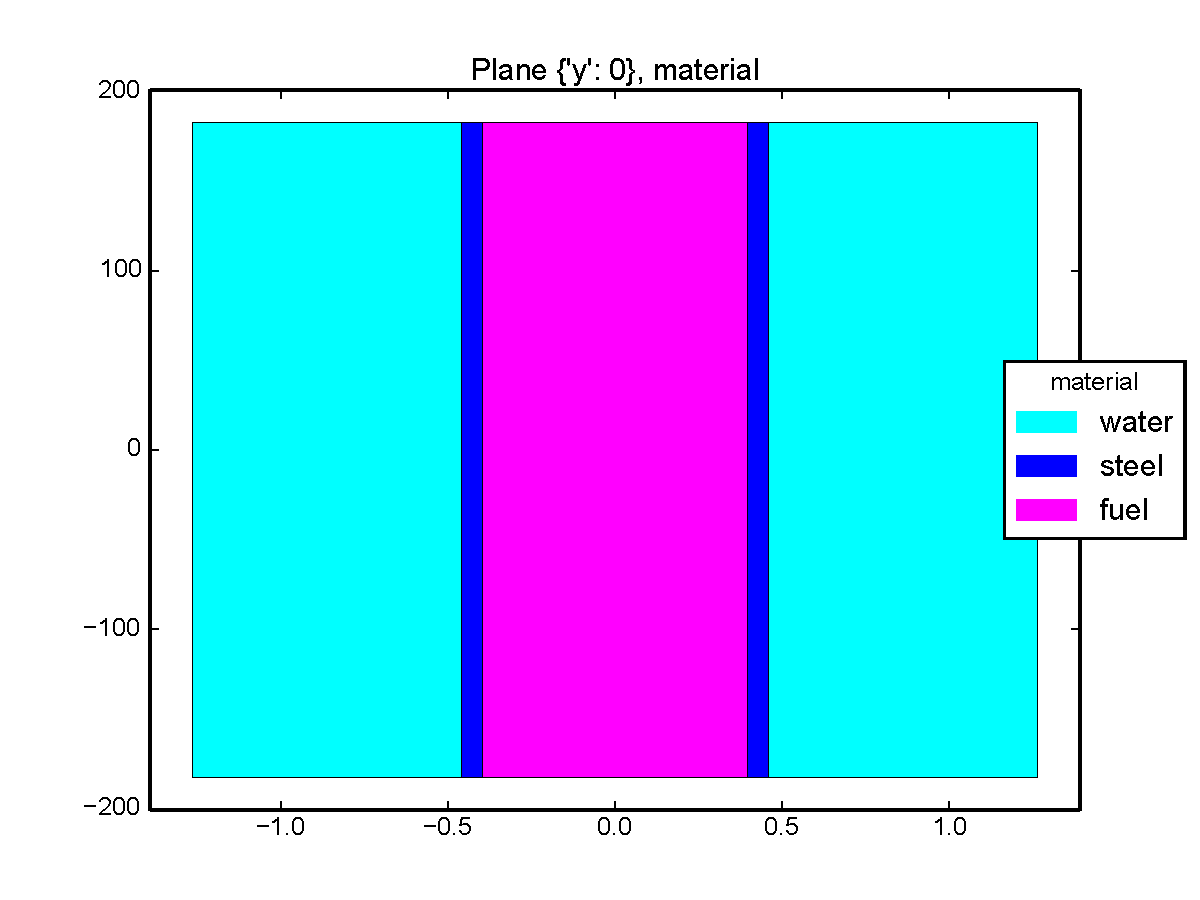
\includegraphics[width=\textwidth]{examples/geom1_py.pdf}
    \end{columns}
\end{frame}

\begin{frame}[fragile]
    \frametitle{System variables}
    \inputminted[frame=single,fontfamily=tt,fontsize=\scriptsize]{python}{examples/geom2.py}
\end{frame}

\begin{frame}\frametitle{System variables: plot}
    \begin{columns}
        \column{0.5\textwidth}
        {\tiny density at plane y=0}
        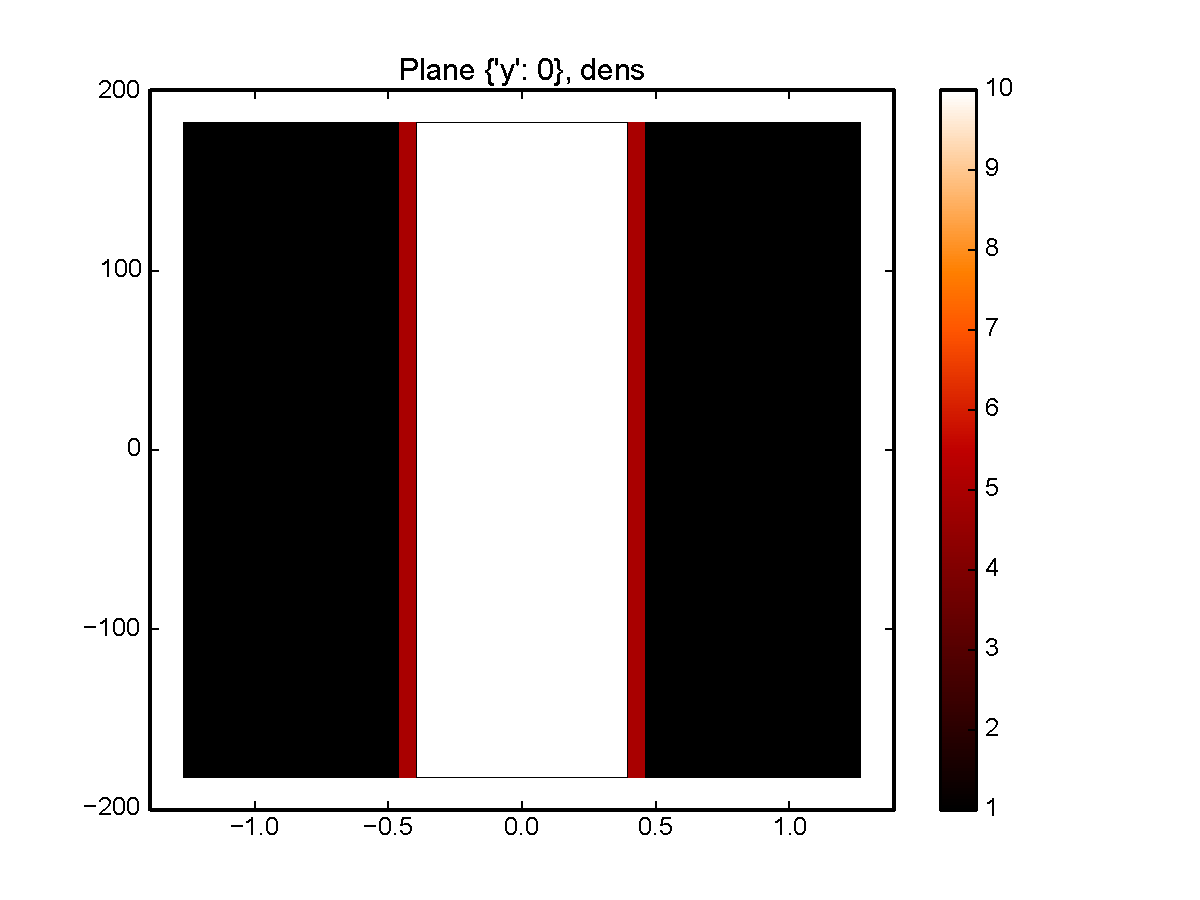
\includegraphics[width=\textwidth]{examples/geom2_d.pdf}
        \column{0.5\textwidth}
        {\tiny temperature at plate y=0}
        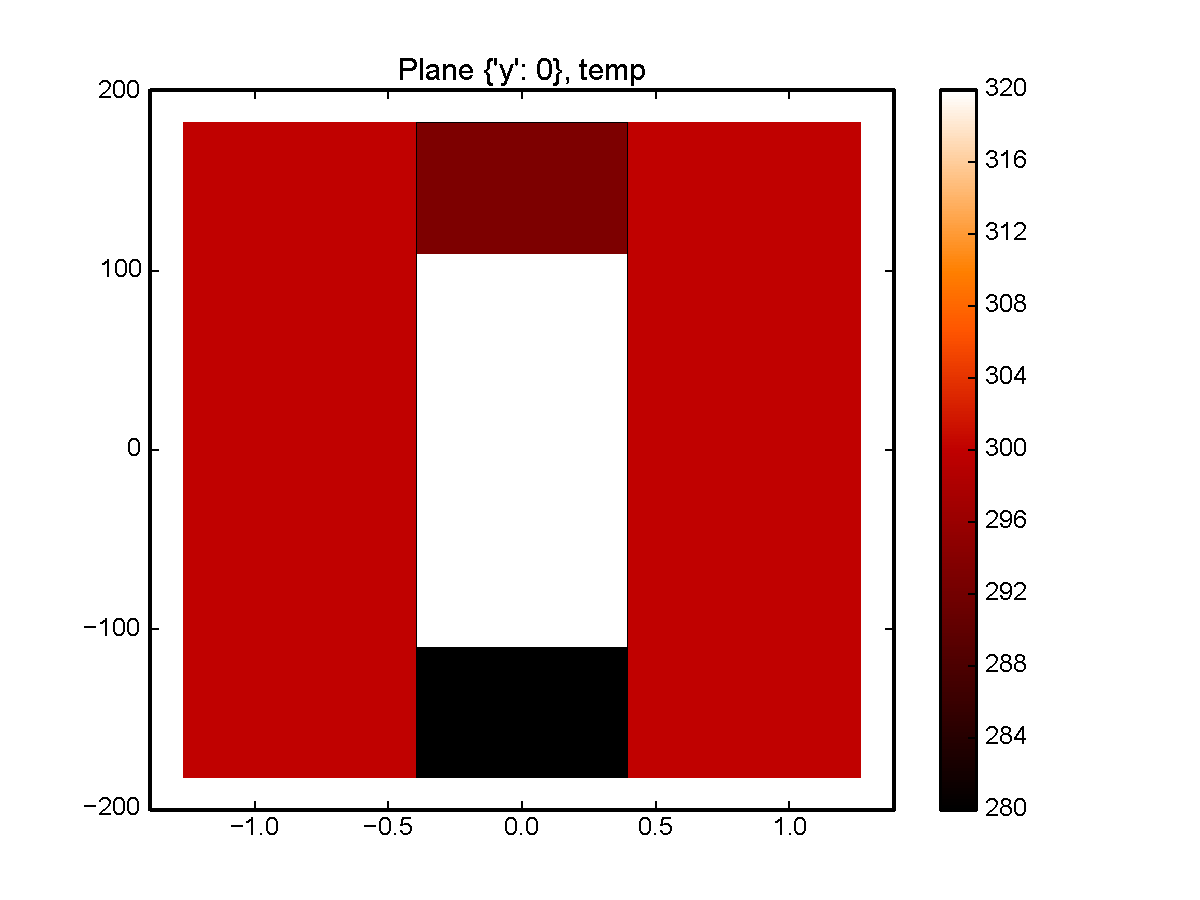
\includegraphics[width=\textwidth]{examples/geom2_t.pdf}
    \end{columns}
\end{frame}

\begin{frame}[fragile]
    \frametitle{Geometry II}
    \inputminted[frame=single,fontfamily=tt,fontsize=\footnotesize]{python}{examples/geom3.py}
\end{frame}

\begin{frame}\frametitle{Geometry II: plots}
    \begin{columns}
        \column{0.3\textwidth}
            {\tiny z plane}
            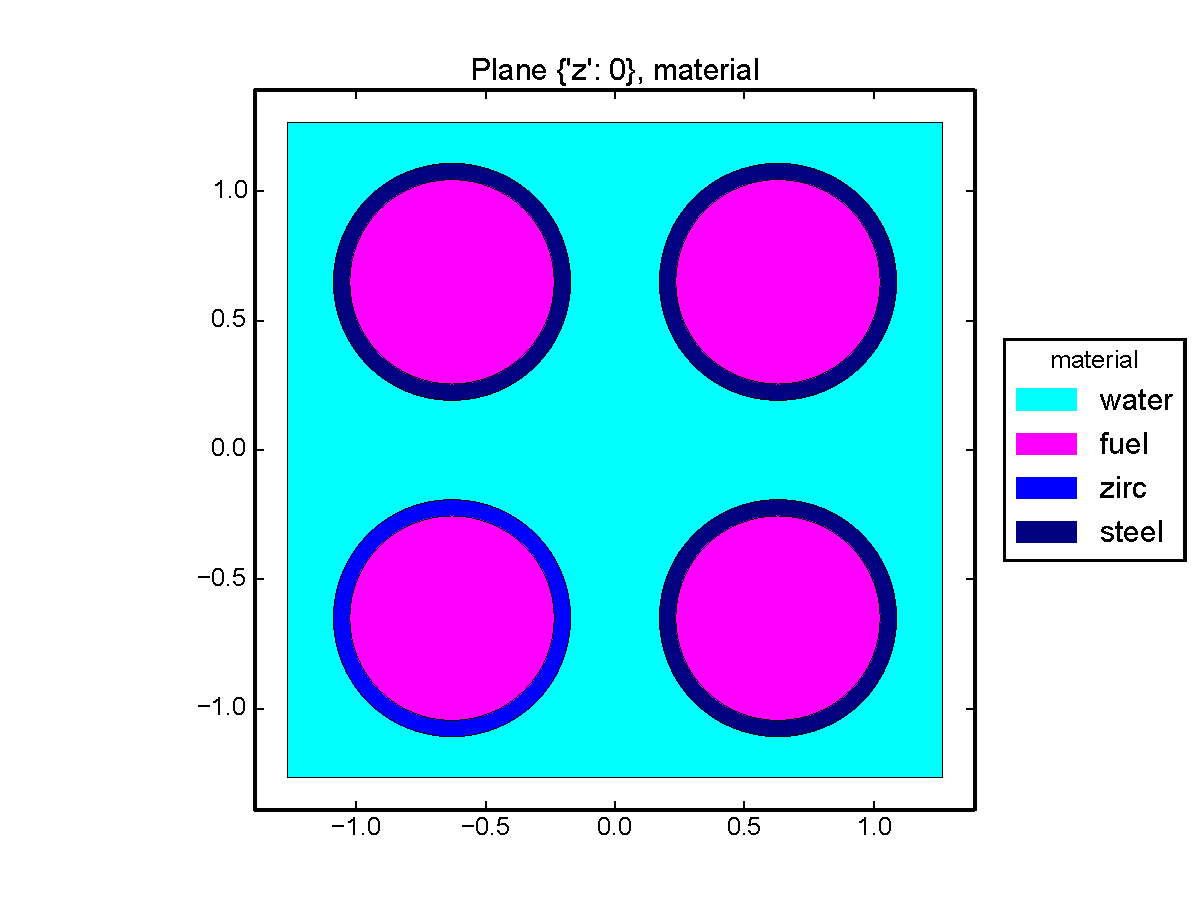
\includegraphics[width=\textwidth]{examples/geom3_pz.pdf}
        \column{0.3\textwidth}
            {\tiny x plane at -1}
            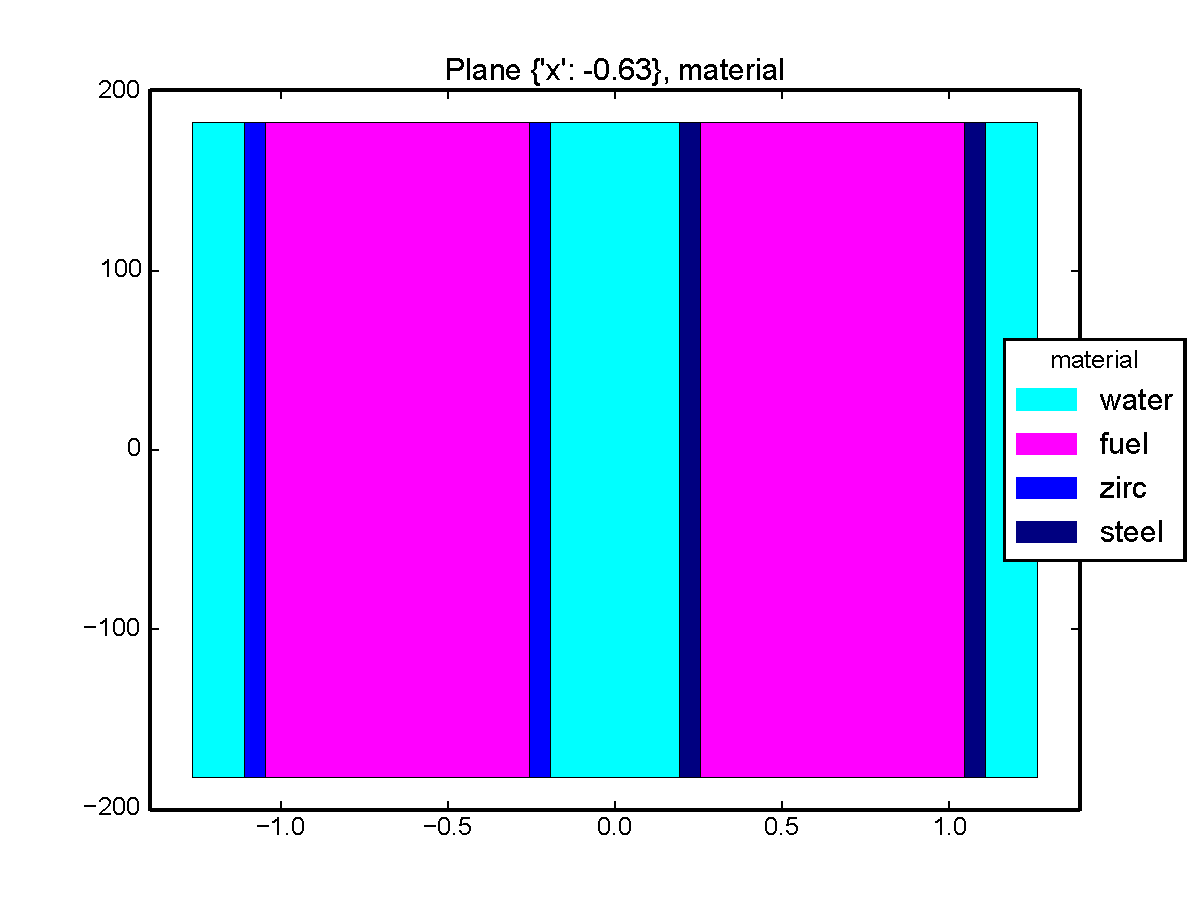
\includegraphics[width=\textwidth]{examples/geom3_px1.pdf}
        \column{0.3\textwidth}
            {\tiny y plane at 1}
            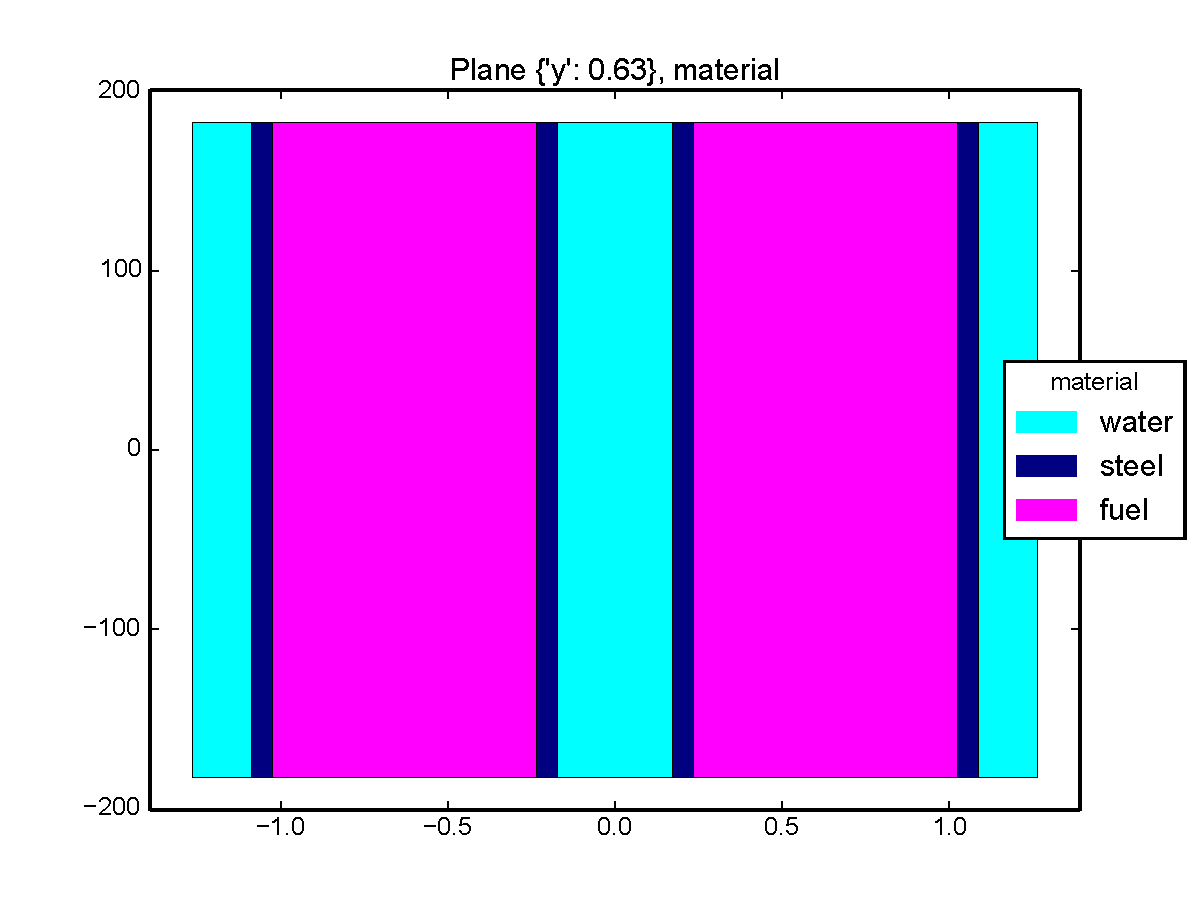
\includegraphics[width=\textwidth]{examples/geom3_py2.pdf}
    \end{columns}
\end{frame}


